%% FX-26: a PLDI-style paper, drafted from the fixpt, kayak and heist
%% repositories. Every number is taken from those repositories; see
%% TODO-paper.md beside this file for what a submission still needs.
\documentclass[acmsmall,screen,review]{acmart}

\usepackage{booktabs}
\usepackage{listings}
\usepackage{tikz}
\usetikzlibrary{positioning,arrows.meta,fit}
\usepackage{amsmath}

\setcopyright{rightsretained}
\acmJournal{PACMPL}
\acmYear{2027}
\acmVolume{11}
\acmNumber{PLDI}
\acmArticle{1}
\acmMonth{6}
\acmDOI{10.1145/nnnnnnn}

\begin{CCSXML}
<ccs2012>
<concept><concept_id>10011007.10011006.10011008.10011024</concept_id>
<concept_desc>Software and its engineering~Language features</concept_desc>
<concept_significance>500</concept_significance></concept>
<concept><concept_id>10011007.10011006.10011041</concept_id>
<concept_desc>Software and its engineering~Compilers</concept_desc>
<concept_significance>500</concept_significance></concept>
<concept><concept_id>10003752.10010124.10010125.10010130</concept_id>
<concept_desc>Theory of computation~Type structures</concept_desc>
<concept_significance>300</concept_significance></concept>
</ccs2012>
\end{CCSXML}
\ccsdesc[500]{Software and its engineering~Language features}
\ccsdesc[500]{Software and its engineering~Compilers}
\ccsdesc[300]{Theory of computation~Type structures}
\citestyle{acmauthoryear}

\lstdefinelanguage{fx}{
  morekeywords={define,lambda,let,letrec,if,begin,plambda,poly,subr,maxeff,
    pure,spin,mu,oneof,allof,sumof,productof,tagcase,par,spawn,with,
    module,stage,attempt,pselect,race,the,loop,requires,ensures,macro,bind},
  sensitive=true,
  morecomment=[l]{;},
  morestring=[b]",
  alsoletter={-,*,?,!,@,:,>,<,=,\#},
}
\lstset{
  language=fx,
  basicstyle=\ttfamily\footnotesize,
  keywordstyle=\bfseries,
  commentstyle=\color{black!60},
  columns=fullflexible,
  keepspaces=true,
  showstringspaces=false,
  xleftmargin=1em,
  aboveskip=0.6em,
  belowskip=0.6em,
  breaklines=true,
  breakatwhitespace=true,
}
\lstdefinestyle{out}{language={},basicstyle=\ttfamily\footnotesize\color{black!75}}
\lstdefinestyle{rust}{language={},basicstyle=\ttfamily\footnotesize}

\newcommand{\cd}[1]{\texttt{#1}}
\newcommand{\fx}{FX-26}
\newcommand{\judge}[4]{#1 \vdash #2 : #3 \mathrel{!} #4}
\newcommand{\frv}{\mathrm{frv}}
\newcommand{\fv}{\mathrm{fv}}

\begin{document}

\title{FX-26: Effects That Something Acts On}
\subtitle{A self-hosted type-and-effect language, its compilers, and what its
effects license}

\author{The Fixpt Team}
\affiliation{\institution{(author list and affiliations to be supplied)}\city{---}\country{---}}

\begin{abstract}
Type-and-effect systems began with FX-87, whose types said which regions
of memory a procedure reads, writes and allocates. Most of what followed
either kept effects as an analysis the programmer never sees, or
re-founded them on handlers. We report on \fx, a language that returns
to the original design---effects on regions, written in signatures,
with masking---and asks a different question of every effect it has:
\emph{what acts on it?}

\fx{} extends the FX line with a termination effect checked by the
size-change principle, control effects for both undelimited and delimited
continuations, effects for message passing, write-once cells,
nondeterminism and I/O, equi-recursive types with untagged unions and
intersections, first-class modules with dependent procedure types, and
hygienic macros whose signatures are binding-structure types. Each effect
is a \emph{licence}: the compiler deletes and specialises code by it, the
REPL runs code speculatively on every keystroke by it, \cd{par} runs
branches in parallel by it, \cd{race} and \cd{attempt} cancel
computations by it, and a translator to Rust chooses between a plain
function, a \cd{Result}-returning function and an \cd{async} function
by it.

The implementation is 87,000 lines of \fx{}---reader, checker, two
compilers, and arm64 and x86-64 code generators---kept in lockstep with
an independent implementation in Rust that bootstraps it. A further
38,000 lines of applications (an editor, a Scheme, an SMT solver, a
relational model finder, a bounded model checker, a control-flow
analysis) and 50,000 lines in an \fx{} subset that compiles to safe
Rust---its own compiler, which reproduces itself byte for byte, and a
second implementation of the language---serve as evidence. We describe the design, say for each effect what consumes it and
where nothing yet does, report what the effect system cost and bought
in those programs, and give an account of its soundness: a paper proof of the memory fragment,
and eighteen holes found and closed along the way, most of them in the
termination effect.
\end{abstract}

\keywords{type-and-effect systems, regions, effect masking, termination,
control effects, self-hosting compilers, hygienic macros, first-class modules}

\maketitle

%% ------------------------------------------------------------------
\section{Introduction}
\label{sec:intro}

In 1987 the FX-87 language~\cite{fx87,lucassen-gifford} gave procedures
types of the form \cd{(subr $F$ ($T \ldots$) $T$)}: a procedure from
arguments to a result, with a \emph{latent effect} $F$ describing which
regions of the store a call may read, write or allocate in. Two ideas
from that design became permanent parts of the field. One is the effect
discipline itself~\cite{talpin-jouvelot}. The other is \emph{masking}:
an effect on a region that no one outside an expression can name is
unobservable and may be dropped, which is the observation region-based
memory management~\cite{tofte-talpin} is built on.

The languages in everyday use that track effects today mostly took
other roads: effects as rows of handler
operations~\cite{koka,plotkin-pretnar,ocaml5}, as
capabilities~\cite{effekt,capturing-types}, or as ownership and
borrowing~\cite{rustbelt}. FX's own road---effects \emph{on regions},
\emph{declared in signatures}, with subeffecting and masking---was left
after FX-91~\cite{fx91}. This paper reports what happens when one walks
it again with thirty-five more years of type-system results in hand, and
with a rule of design that the original did not have:
\begin{quote}
\emph{An effect is in the language only if something acts on it.}
\end{quote}

\paragraph{What ``acts on'' means.} Every effect in every effect system
is acted on in a trivial sense: the type checker rejects a program
whose body does more than its signature says. We do not count that.
We say a component \emph{acts on} an effect atom $a$ when it makes a
decision about a program---to transform it, to run it early, to run
parts of it concurrently, to abandon it part-way, to choose a
representation for it---and that decision is correct only because the
program's effect does, or does not, contain $a$. The effect is the
\emph{input to a decision someone other than the type checker makes}.
We call such a decision procedure a \emph{consumer} of the effect, and
the pattern \emph{effects as licences}: an effect bound is a
permission, established by the checker, for a consumer to do something
that would otherwise be unsound.

Table~\ref{tab:consumers} applies the test to each effect \fx{} has.
It is the paper's thesis in one table, and we have tried to fill it in
without flattery. Most rows have several consumers. Some do not. We
found no consumer that tells most of the sixteen kinds of I/O effect
apart: parallel evaluation, the REPL and the cancellation forms treat
every I/O effect alike, so the kinds presently serve documentation and
search only. The nondeterminism effect has one thin consumer. By the
paper's own rule these are the weakest parts of the design, and we say
so here rather than leave a reviewer to find it.

\begin{table}[t]
\caption{What acts on each effect, beyond the subsumption check.
Section numbers say where each consumer is described.}
\label{tab:consumers}
\small
\begin{tabular}{@{}p{0.23\linewidth}p{0.73\linewidth}@{}}
\toprule
effect & consumers, and the decision each makes\\
\midrule
read, write, allocate\newline on a region &
\emph{masking}: drop the effect where the region is private (\S\ref{sec:core});
\emph{parallel evaluation}: branches may run concurrently if their effects do not conflict (\S\ref{sec:conc});
\emph{speculation}: the REPL may run code early (\S\ref{sec:licences});
\emph{cancellation}: a computation that writes nothing outside itself may be abandoned (\S\ref{sec:conc});
\emph{narrowing}: a fact learned by a test survives until a write to the region it was read through (\S\ref{sec:core});
\emph{compiler}: allocation in an arena region is an inline pointer bump (\S\ref{sec:compiler-licence})\\[3pt]
capture or invoke a\newline continuation &
\emph{Rust translation}: chooses plain, \cd{Result}-returning or \cd{async} function (\S\ref{sec:kayak});
\emph{arenas}: a region may be freed on exit only if no captured continuation can re-enter it;
\emph{parallel evaluation} and \emph{cancellation}: refuse code that can jump out\\[3pt]
may not terminate &
\emph{code removal}: an unused call is deleted only if it is pure \emph{and} terminates (\S\ref{sec:compiler-licence});
\emph{specifications}: any pure, terminating procedure may be used in a logical formula;
\emph{speculation}: needs a step budget where present\\[3pt]
send, receive; wait on or fill a write-once cell &
\emph{parallel evaluation}; \emph{speculation}; \emph{cancellation};
\emph{Rust translation}: closure types gain \cd{Send + Sync}\\[3pt]
read or write a named global variable &
\emph{redefinition}: which earlier definitions a redefinition invalidates (\S\ref{sec:core});
\emph{compiler}: one guarded entry per procedure body where globals cannot change under it (\S\ref{sec:compiler-licence});
\emph{modules}: loading may be shared because it only reads globals (\S\ref{sec:macros})\\[3pt]
I/O (sixteen kinds) &
\emph{parallel evaluation}, \emph{speculation}, \emph{cancellation}: all refuse or sequence any I/O.
\textbf{Gap:} nothing we found distinguishes most kinds from one another\\[3pt]
nondeterminism &
\emph{speculation} refuses it. \textbf{Gap:} otherwise it is a statement to the reader that results may vary between runs\\[3pt]
generates code at run time &
\emph{speculation} refuses it\\
\bottomrule
\end{tabular}
\end{table}

\paragraph{The language.} \fx{} is a statically typed, strict,
impure functional language. Its concrete syntax is the parenthesised
prefix notation of Lisp (\S\ref{sec:overview} explains how to read it);
nothing in the design depends on that choice. Definitions carry
explicit signatures, and types inside a definition are found by
bidirectional checking. Its effects are finite sets of atoms. Beyond FX-87's \cd{read},
\cd{write} and \cd{alloc} on regions, it has: \cd{spin}, the effect of
code that may not terminate, checked by the size-change
principle~\cite{size-change}; \cd{goto} and \cd{comefrom}, the control
effects of Jouvelot and Gifford~\cite{jouvelot-gifford}, extended to
delimited continuations; \cd{send}, \cd{receive}, \cd{await},
\cd{init} and \cd{nondet} for processes with separate heaps and
write-once cells; a family of sixteen \cd{io} effects; and reads and
writes of named global variables. Its types include equi-recursive
\cd{mu} types compared coinductively~\cite{amadio-cardelli,brandt-henglein},
untagged unions narrowed by tests~\cite{typed-scheme}, intersections of
procedure types, first-class modules with dependent procedure types
after Sheldon and Gifford~\cite{sheldon-gifford}, and macros whose
signatures are Herman's binding-structure types~\cite{herman-thesis},
inferred for macros defined by pattern and template.

\paragraph{The evidence.} A language design paper stands on what was
built with the language. We have three bodies of code
(\S\ref{sec:eval}):
\begin{itemize}
\item \textbf{Fixpt}, the implementation. Its front end---reader, parser,
  module loader, checker, macro expander, a compiler to threaded code,
  a compiler to register code, and code generators for arm64 and
  x86-64---is 87,071 lines of \fx{} in 238 files. An independent
  implementation of the same pipeline in Rust bootstraps it, and the two
  are held in \emph{lockstep}: both checkers run on every program and
  must agree, and both compilers' output is compared.
\item \textbf{Heist}, 38,202 lines of application programs written by
  a client project separate from the language's own: an
  Emacs-style text editor, an implementation of standard Scheme, a
  CDCL SAT and SMT solver, a relational model finder after Alloy, a
  bounded model checker, and a control-flow analysis.
\item \textbf{Kayak}, which defines KFX, a subset of \fx{} in which every
  construct maps to safe Rust, with a translator written in KFX that
  reproduces its own Rust output byte for byte; and, written in KFX, a
  second implementation of \fx{} with its own checker,
  compilers and collector (50,600 lines of KFX in all).
\end{itemize}

\paragraph{Contributions.}
\begin{enumerate}
\item The design of \fx{} (\S\ref{sec:overview}--\S\ref{sec:core}): a
  region-and-effect language in the FX tradition with termination,
  control, communication and I/O as effects, a single masking rule that
  serves all of them, and structural recursive, union and intersection
  types under bidirectional checking.
\item \emph{Effects as licences} (\S\ref{sec:licences}): six consumers
  of effect information beyond the checker---an optimising compiler,
  a speculating REPL, deterministic \cd{par}, cancellation in \cd{race}
  and \cd{attempt}, staged code, and a verifier---each stated as a
  condition on effects.
\item A translation of effects to Rust (\S\ref{sec:kayak}) in which the
  ``colour'' of a function is read off its latent effect: \cd{goto}
  selects \cd{Result}, \cd{comefrom} selects \cd{async}, and effects that
  cross process boundaries select \cd{Send + Sync}; with a compiler
  that bootstraps through it.
\item Typed hygienic macros in a typed language (\S\ref{sec:macros}),
  with signatures written as shapes and binding facts, inferred for pattern-and-template macros, and checked at definitions and uses.
\item A self-hosted implementation kept in lockstep with a second one
  (\S\ref{sec:impl}), and an experience report (\S\ref{sec:eval}) from 125,000
  lines of \fx{}, including counts of how effects are actually
  written in application code.
\item An account of soundness as practised (\S\ref{sec:soundness}): what
  is proved, what is conjectured, the eighteen holes found, and why
  eight of them were in one effect.
\end{enumerate}

\paragraph{What this paper is not.} It is not a performance
evaluation: no \fx{} program has been timed against another language's
implementation under controlled conditions, and we make no claim about
its speed relative to any. It is not a soundness proof: the metatheory
is on paper, for a fragment. \fx{} is eight weeks of design old at the
time of writing and several features are prototypes. The paper's
evidence is that the design could be implemented in itself, twice
over, and used for sizeable programs; \S\ref{sec:eval} reports that
experience and says at its head what may and may not be concluded
from it.

%% ------------------------------------------------------------------
\section{FX-26 by Example}
\label{sec:overview}

\paragraph{Reading the notation.} Programs and types are written in
prefix form: \cd{(f a b)} applies \cd{f}, and
\cd{(define $x$ $T$ $e$)} defines $x$ with type $T$ and value $e$.
The type \cd{(subr $F$ ($T_1 \ldots$) $T$)} is a function from
$T_1 \ldots$ to $T$ whose calls have effect $F$; \cd{(maxeff $F_1$
$F_2$)} is the union of two effects and \cd{pure} is none. A name
beginning \cd{@} is a region: a static name for a set of mutable
locations. \cd{(ref int @a)} is a mutable cell holding an integer in
region \cd{@a}, made by \cd{new} and used by \cd{get} and \cd{set}.
\cd{(the $T$ $e$)} is a type ascription, \cd{letrec} binds local
recursive functions, and \cd{\#u} is the unit value. After each
definition or expression the system prints its value, its type, and
after \cd{!} its effect.


\paragraph{Masking: local state is an implementation detail.}
The following procedure allocates a reference cell and writes it a
hundred times.

\begin{lstlisting}
(define sum-to (subr pure (int) int)
  (lambda (n)
    (let ((acc (the (ref int @a) (new 0))))
      (letrec ((go (subr (maxeff (read @a) (write @a)) (int) unit)
                 (lambda (i) (if (<= i 0) #u (begin (set acc (+ (get acc) i)) (go (- i 1)))))))
        (begin (go n) (get acc))))))
(sum-to 100)
\end{lstlisting}
\begin{lstlisting}[style=out]
sum-to : (subr pure (int) int) ! pure
5050 : int ! (read (globals sum-to))
\end{lstlisting}
The signature of
\cd{sum-to} says \cd{pure}, and the checker accepts it: the cell lives
at region \cd{@a}; no free variable of the \cd{let} has a type
mentioning \cd{@a}, and neither does its result; so the allocation,
reads and writes at \cd{@a} are \emph{masked}. Two further things are
visible. The inner loop \cd{go} needs no \cd{spin} in its effect,
because the checker sees \cd{i} count down under a test that bounds it
below. And the call's one remaining effect is that it read a global
variable: globals form a region that appears only in effects and is
never masked, which is what lets an interactive system know which
earlier results a redefinition invalidates.

\paragraph{Termination is an effect.} A recursion the checker cannot
see end must say \cd{spin}, and the refusal explains itself:
\begin{lstlisting}
(define steps (subr pure (int) int)
  (letrec ((go (subr pure (int int) int)
             (lambda (n k) (if (= n 1) k
               (go (if (= 0 (remainder n 2)) (quotient n 2) (+ (* 3 n) 1)) (+ k 1))))))
    (lambda (n) (go n 0))))
\end{lstlisting}
\begin{lstlisting}[style=out]
collatz.fx:3:14: `go` is declared a (subr pure (int int) int): a (subr pure (int int) int)
is expected here, and this is a (subr spin (int int) int)
  beyond what is expected, it has spin; it may not end: nothing smaller, or related, is
  passed by the call of `go` in `go` (it counts up, but nothing fixed bounds the count above)
\end{lstlisting}

\paragraph{Control is typed.} Capturing a continuation has a
\cd{comefrom} effect and invoking one a \cd{goto}, each on a
region~\cite{jouvelot-gifford}. They are masked like memory effects, so
a procedure that uses an escape internally is still pure. Below,
\cd{cwcc} (``call with current continuation'') passes its argument the
rest of the computation as a function \cd{k}; calling \cd{k} with 41
makes 41 the result of the \cd{cwcc} expression:
\begin{lstlisting}[style=out]
42 : int ! pure                  ; (+ 1 (cwcc (lambda (k) (k 41))))
\end{lstlisting}

\paragraph{Structural types.} Recursive types are written in place and
compared as the infinite trees they unfold to. A union needs no tags
where a run-time test tells its members apart; a test narrows.
\begin{lstlisting}
(define leaves (subr pure ((mu t (oneof int (listof t acyclic)))) int)
  (letrec ((leaves (subr pure ((mu t (oneof int (listof t acyclic)))) int)
             (lambda (x)
               (if (int? x) 1
                   (if (null? x) 0 (+ (leaves (car x)) (leaves (cdr x))))))))
    leaves))
\end{lstlisting}
The type says a tree is an integer or a list of trees (\cd{car} and
\cd{cdr} are a list's head and tail). The test \cd{int?} narrows
\cd{x}; the tail \cd{(cdr x)} is a list of trees and so,
by subtyping through the \cd{mu}, a tree; and \cd{leaves} is \cd{pure}
because a list at the region \cd{acyclic} is finite, so descent into
its parts terminates. The three features---regions, recursive subtyping
and the termination effect---meet in one line.

\paragraph{Effects decide what may run in parallel, and when.}
\cd{par} evaluates its branches in parallel and is refused when their
effects interfere:
\begin{lstlisting}
(define xs (arrayof int @x) (make-array 3 0))
(par ((a (begin (array-set! xs 0 1) 0))
      (b (array-ref xs 0)))
  (+ a b))
\end{lstlisting}
\begin{lstlisting}[style=out]
par-interfere.fx:5:1: `par`'s branches interfere: one has (write @x) and another
(read @x), so the answer could depend on which runs first
\end{lstlisting}
The same information drives the REPL, which checks each expression as it
is typed and evaluates a finished one \emph{before} the user presses
Enter, if and only if its effect is one that cannot be observed:
\begin{lstlisting}[style=out]
fx26> (car (cons 1 #t))          ; = 1
fx26> (set c 5)                  ; not run early: it may (write @c)
\end{lstlisting}
The reader that decides when a form is complete is itself an \fx{}
program run on every keystroke under the same rule.

%% ------------------------------------------------------------------
\section{The Core Language}
\label{sec:core}

\fx's kernel starts from KFX, the calculus of the PLDI~'89 control-effects
paper~\cite{jouvelot-gifford}: kinds \cd{region}, \cd{effect} and
\cd{type}; effects \cd{pure}, \cd{(read $R$)}, \cd{(write $R$)},
\cd{(alloc $R$)} and \cd{maxeff}; types \cd{subr}, \cd{poly} and
\cd{ref}. Figure~\ref{fig:grammar} gives the present grammar of
descriptions in outline, and Figure~\ref{fig:rules} the rules the rest
of this section explains.

\begin{figure}[t]
\small
\[
\begin{array}{rcl}
\kappa &::=& \cd{region} \mid \cd{place} \mid \cd{effect} \mid \cd{type}
   \mid \cd{data} \mid \cd{sendable} \mid \cd{size} \mid \cd{(=> ($\kappa^+$) $\kappa$)}\\[2pt]
R &::=& \cd{@}n \mid r \mid \cd{heap} \mid \cd{const} \mid \cd{acyclic}
   \mid \cd{(const $p$)} \mid \cd{(acyclic $p$)}\\[2pt]
F &::=& \cd{pure} \mid \cd{(maxeff $F \ldots$)} \mid e
   \mid \cd{(read $R$)} \mid \cd{(write $R$)} \mid \cd{(alloc $R$)}
   \mid \cd{(init $R$)} \mid \cd{(await $R$)}\\
  &\mid& \cd{(goto $R$)} \mid \cd{(comefrom $R$)}
   \mid \cd{(send $R$)} \mid \cd{(receive $R$)}\\
  &\mid& \cd{(read (globals $g \ldots$))} \mid \cd{(write (globals $g \ldots$))}
   \mid \cd{spin} \mid \cd{nondet} \mid \cd{(io $k$)} \mid \cd{stage}\\[2pt]
T &::=& \cd{int} \mid \cd{nat} \mid \cd{bool} \mid \cd{unit} \mid \cd{void}
   \mid \cdots \mid t
   \mid \cd{(subr $F$ ($T \ldots$) $T$)}
   \mid \cd{(poly (($x\ \kappa$)$\ldots$) $T$)}\\
  &\mid& \cd{(ref $T$ $R$)} \mid \cd{(listof $T$ $R$)}
   \mid \cd{(arrayof $T$ $R$)} \mid \cd{(icell $T$ $R$)}
   \mid \cd{(addr $T$ $R$)} \mid \cd{(inbox $T$ $R$)}\\
  &\mid& \cd{(sumof ($\ell\ T$)$\ldots$)} \mid \cd{(productof ($\ell\ T$)$\ldots$)}
   \mid \cd{(oneof $T \ldots$)}\\
  &\mid& \cd{(anyof $T \ldots$)}
   \mid \cd{(allof $T \ldots$)} \mid \cd{(mu $t$ $T$)}
   \mid \cd{(prompt-tag $A$ $H$ $D$ $R$)}\\
  &\mid& \cd{(moduleof $\mathit{item} \ldots$)} \mid \cd{(select $m$ $t$)}
\end{array}
\]
\Description{Grammar of kinds, regions, effects and types.}
\caption{Descriptions of \fx{} in outline: kinds $\kappa$, regions $R$,
effects $F$ and types $T$. $r$, $e$, $t$ and $p$ range over region,
effect, type and place variables; $k$ over sixteen I/O kinds. Fixed-width
integers, floats, strings, byte vectors, flat arrays, bloblets,
variadic procedures and generative types are omitted.}
\label{fig:grammar}
\end{figure}

\begin{figure}[t]
\small
\[
\begin{array}{c}
\dfrac{\judge{\Gamma, x_i{:}T_i}{b}{T}{F}}
      {\judge{\Gamma}{\cd{(lambda ($x_i \ldots$) $b$)}}{\cd{(subr $F$ ($T_i \ldots$) $T$)}}{\cd{pure}}}
\;\textsc{(Abs)}
\\[14pt]
\dfrac{\judge{\Gamma}{f}{\cd{(subr $F$ ($T_i \ldots$) $T$)}}{F_0}\quad
       \judge{\Gamma}{a_i}{T_i}{F_i}}
      {\judge{\Gamma}{\cd{($f\ a_i \ldots$)}}{T}{F_0 \cup \bigcup_i F_i \cup F}}
\;\textsc{(App)}
\\[14pt]
\dfrac{\judge{\Gamma}{e}{T}{F}\quad T \le T'\quad F \subseteq F'}
      {\judge{\Gamma}{e}{T'}{F'}}
\;\textsc{(Sub)}
\qquad
\dfrac{\judge{\Gamma}{e}{T}{F}\quad
       r \notin \frv(\Gamma|_{\fv(e)}) \cup \frv(T)}
      {\judge{\Gamma}{e}{T}{F \setminus \{\,a(r) \mid a \in \mathcal{M}\,\}}}
\;\textsc{(Mask)}
\\[14pt]
\dfrac{\judge{\Gamma}{e_i}{T_i}{F_i}\quad
       \mathit{local}(F_i)\quad
       F_i \mathrel{\#} F_j\ (i \ne j)\quad
       \judge{\Gamma, x_i{:}T_i}{b}{T}{F}}
      {\judge{\Gamma}{\cd{(par (($x_i\ e_i$)$\ldots$) $b$)}}{T}{F \cup \bigcup_i F_i}}
\;\textsc{(Par)}
\end{array}
\]
\[
\begin{array}{l}
\mathcal{M} = \{\cd{read}, \cd{write}, \cd{alloc}, \cd{init}, \cd{await},
  \cd{goto}, \cd{comefrom}\}\\[3pt]
\mathit{licensed}_O(F) \iff \forall a \in F.\ a = \cd{(alloc $R$)} \lor
  (a = m(R) \land m \in \mathcal{M} \land R \in O)
\end{array}
\]
\Description{Typing rules Abs, App, Sub, Mask and Par.}
\caption{Selected rules. Effects are finite sets of atoms. \textsc{(Mask)}
applies at every expression that combines effects; atoms with no
region---\cd{spin}, \cd{nondet}, \cd{(io $k$)}---and effects on globals
and on \cd{const} are never in its scope. $\mathit{local}(F)$ holds when $F$ has no \cd{goto} or \cd{comefrom};
$F_i \mathrel{\#} F_j$ is non-interference (\S\ref{sec:conc}); $\mathit{licensed}_O$ is the licence
of a driver owning regions $O$ (\S\ref{sec:licences}); an effect variable
is never licensed.}
\label{fig:rules}
\end{figure}

\subsection{Effects, Subeffecting and Masking}

An effect is a finite set of atoms; \cd{maxeff} is union and \cd{pure}
the empty set. Subeffecting is inclusion, extended by a small order
among I/O kinds. A procedure type is contravariant in its parameters
and covariant in its result and its latent effect.

The masking rule of Figure~\ref{fig:rules} is applied implicitly at
every subexpression that combines effects, as FX-87's reference
implementation did. It has one premise: the region occurs neither in
the types of the expression's free variables nor in the expression's
own type. An earlier formulation followed FX-87 in also dropping reads
and writes on a region that the \emph{result} mentions (keeping only
allocation). That was unsound once regions carried the property
\cd{acyclic}: a procedure that tied the structure it returned into a
cycle could declare only \cd{(alloc $r$)}, be instantiated at an
acyclic region, and make a cyclic ``acyclic'' list on which a \cd{pure}
recursion then looped. The hole was accepted by both checkers and found
only when an application author asked how soundness was being tested.
The rule now masks only regions in neither position.

The same rule serves control. A \cd{goto} or \cd{comefrom} on $r$ is
masked when the expression neither imports nor returns values whose
types mention $r$---for \cd{goto} this is strictly more demanding than
FX-87's memory rule, and we keep the seven conformance cases of the
PLDI~'89 paper as tests, with deliberate mutations of the checker to
show each case discriminates. A masked \cd{await} leaves a \cd{spin}
behind, since a wait on a private cell that nothing fills does not
terminate.

Region binders---\cd{letregion}, and the arena and reap forms
\cd{letrena} and \cd{letreap} that also free their storage---require
that the body's value not mention the region and that no \cd{comefrom}
survive in its masked effect: a continuation captured inside must not
re-enter a freed arena.

\subsection{Globals as a Region}

Naming a global $g$ has effect \cd{(read (globals $g$))}. The region
\cd{@globals} stands for every global, past and future, and absorbs
individual reads. Because signatures are written, a definition whose
body calls library procedures would have to list them; the form
\cd{define*} computes the set of globals read and leaves the rest of
the signature as written. It was by far the most used definition form
in application code (\S\ref{sec:heist}).

Tracking globals is what makes redefinition in a session sound: when
\cd{f} is redefined at a different type, every definition whose effect
reads \cd{f} is marked broken, with the reason, rather than left to
fail or silently keep the old code.

\subsection{Termination}
\label{sec:spin}

\cd{spin} is an atom with no region, so nothing masks it. A call within
a recursive group has \cd{spin} unless the group passes the size-change
test of Lee, Jones and Ben-Amram~\cite{size-change}, with three
measures: \emph{parts} (the payload bound by a pattern match on a sum, a field, or
the head or tail of a list at an \cd{acyclic} region);
\emph{down} (an integer decreased by a literal under a test bounding it
below); and \emph{up} (increased by a literal under a bound above).
This is enough for list and tree traversals, counting loops, mutual
recursion such as \cd{even?}/\cd{odd?}, and Ackermann's function, all
at \cd{pure}. It does not see through lists at writable regions,
through a test such as \cd{(= n 0)} alone, or through a part reached
via another procedure's parameter.

Recursion is not the only way to loop, and the remaining sources of
\cd{spin} are where most of our soundness holes were
(\S\ref{sec:soundness}). \cd{spin} is also charged for self-application
through a type recursive in a parameter position; for a procedure
stored in mutable storage at a region its own latent effect reads
(recursion through the store); for a procedure that reaches itself through a global;
and for \cd{cwcc} unless its receiver only calls the continuation while
the capture is live.

There is no separate cycle analysis. The evidence that a list is finite
is that it lives at a region nothing may write: \cd{acyclic} is a
frozen region, and freezing is a region operation (\cd{letfreeze}).

\subsection{Types}

\paragraph{Recursive types.} A type is a graph. \cd{(mu $t$ $T$)} needs
no name and no fold or unfold; subtyping compares graphs, assuming each
pair already under comparison, in the manner of Amadio and
Cardelli~\cite{amadio-cardelli} with the rule structure of Brandt and
Henglein~\cite{brandt-henglein} run as an algorithm with one trail.
Sums admit width and depth subtyping; products depth only. Sums and
products are immutable and live in no region, a deliberate change from
FX-87, whose mutable \cd{oneof} made its width rule unsound.

\paragraph{Unions and narrowing.} \cd{(oneof $T \ldots$)} is an
untagged union whose members a run-time shape test can tell apart;
\cd{anyof} permits overlap. Predicates carry latent propositions in
their result types, as in Typed Racket~\cite{typed-scheme}:
\cd{(bool (then $P$) (else $Q$))}. What a test established about a
path through the heap lasts until an effect that writes the region read
through or transfers control---the effect system supplies the kill set
that occurrence typing in an impure language otherwise lacks.

\paragraph{Intersections.} \cd{(allof $T \ldots$)} gives one procedure
several types, its body checked against each. A call takes every member
its arguments fit and returns the meet of their results. This lets a
constant folder map closed expressions to closed and open to open from
one body, and lets a \cd{length} procedure be \cd{pure} on acyclic
lists and \cd{spin} on others. With effects, the distributivity
$(A{\to}B)\cap(A{\to}C) \le A{\to}(B\cap C)$ is unsound, as Davies and
Pfenning showed~\cite{davies-pfenning}; we rediscovered this the hard
way (finding F18, \S\ref{sec:soundness}) and now refuse a meet where
the members' results name a region the call allocates in.

\paragraph{Polymorphism and bidirectional checking.} \cd{poly} abstracts
over any kind. Definitions carry signatures; bodies are checked against
them, and types are synthesised locally~\cite{local-type-inference,bidir-survey}.
A \cd{lambda} checked against a \cd{poly} type needs no \cd{plambda},
and a polymorphic operator is instantiated implicitly from its arguments
and expected result. A type binder must be solved; an unconstrained
effect binder is \cd{pure}; an unconstrained region binder is a fresh
region or, where the procedure only allocates and reads pairs there,
\cd{acyclic}---a default prototyped in an application and adopted after
it removed every one of 101 region annotations in one program. Effect
binders may be bounded, \cd{($e$ effect (within $E$))}.

\subsection{Delimited Control}

Prompts, composable continuations and continuation marks follow
the design of Racket's control operators. A \emph{prompt} marks a
point on the stack; a computation may abort to the nearest prompt with
a given tag, or capture the stack up to it as a function. A prompt
tag's type
\cd{(prompt-tag $A$ $H$ $D$ $R$)} fixes the answer type $A$, the
handler's argument $H$, a bound $D$ on what delimited computations may
do, and a region $R$ for its control effects; fixing the answer type in
the tag, as Typed Racket does, rules out answer-type
modification~\cite{danvy-filinski,asai-kameyama} but keeps checking
local. \cd{prompt} is syntax because it delimits: it removes
\cd{(goto $R$)} and \cd{(comefrom $R$)} from its body's effect only if
no free variable of the body, other than the tag, has a type mentioning
$R$.

%% ------------------------------------------------------------------
\section{Effects as Licences}
\label{sec:licences}

This section collects the consumers of effects other than the
subsumption check. Each is a predicate on an effect; when it holds,
some agent may do something.

\subsection{Speculation: the REPL and the Reader}

A \emph{driver} that owns a set $O$ of regions may run code of effect
$F$ without anyone observing that it did when $\mathit{licensed}_O(F)$
(Figure~\ref{fig:rules}): every atom is an allocation, or a memory or
control effect on an owned region. The implementation additionally
admits reads of globals and \cd{spin} (under a step budget), and always
refuses \cd{send}, \cd{receive}, \cd{nondet}, \cd{stage} and \cd{io}.
A licence is masking relative to an observer: what masking proves
unobservable to the rest of the \emph{program}, a licence proves
unobservable to the \emph{user}.

The REPL owns no regions, so it runs a finished expression early
exactly when masking left nothing but allocation. The reader is the
more interesting driver. The REPL feeds each keystroke to a reader
written in \fx{} (which captures continuations and mutates its buffers
freely); it may do so because the reader and parser are module files
parameterised over their regions, so every entry point's latent effect
is licensed for a driver that supplies those regions. No part of this
is trusted: change the reader to write a region it was not given and
the driver's check fails.

\subsection{Determinism and Cancellation}
\label{sec:conc}

Processes have their own heaps and share no mutable memory. The forms
are \cd{spawn}, \cd{send}, \cd{receive}, \cd{self}, I-cells
(write-once cells after I-structures~\cite{i-structures}; \cd{icell-get}
has effect \cd{await} and \cd{icell-put!} \cd{init}), \cd{par},
\cd{pselect} and \cd{race}. Only values of \emph{transmissible} type
cross between processes, a kind between \cd{data} and \cd{type}: no
mutable data, and only procedures whose latent effects any process may
have.

\textsc{(Par)} requires that no branch transfer control out of itself
and that no two branches interfere on regions that may be equal
(Lucassen's rule for region variables~\cite{lucassen-thesis}). The
conflicts are read/write, write/write, write/init, write/await,
send/send, send/receive, receive/receive and I/O with I/O; \cd{init}
commutes with reads and awaits, which is the point of I-cells; an
effect variable conflicts with everything but allocation, \cd{spin} and
\cd{nondet}. The guarantee claimed is: \emph{a computation whose effect
has neither \cd{nondet}, nor a send or await on a region outside it,
gives the same answer on every run.} Two things are documented as
outside the guarantee: which of two failures is reported, and which of
two fills of one I-cell fails.

\cd{race} keeps the first branch to finish and abandons the others;
\cd{(attempt $e$ $h$)} runs $e$ and calls $h$ if it fails;
\cd{attempt-within} adds a time limit. All three are sound only if an
abandoned computation leaves no trace, so they require their bodies to
be \emph{cancellable}: they may read, allocate, await, receive and
spin, and do anything on regions of their own, but not write, fill an
I-cell, send, perform I/O or escape. The editor in Heist relies on this
to make a failing command harmless: a turn is a function from state to
a new state and a list of commands, \cd{attempt} is accepted around it
because its effect is cancellable, and so---in the words of that
project's notes---``rollback is a property of the types, not a
convention.''

\subsection{The Compiler}
\label{sec:compiler-licence}

Compilation is not erasure. In the path that lowers to Scheme, facts
travel with code as quoted \cd{\%fx-note} claims in the style of
an earlier Scheme compiler's annotations~\cite{twobit}, each with a \emph{basis}:
\cd{checked}, \cd{inferred} or \cd{asserted}. Only a checked claim
licenses removing code, a property pinned by a test.
\begin{lstlisting}[style=out]
fx26> (+ 1 2)
; (begin '(%fx-note (integrable %fx26-add) (pure) (basis checked) (because "pure"))
;        (%fx26-add 1 2))
\end{lstlisting}
In the native compilers, types select unchecked instruction sequences
(a call without a closure test; a list's head as one load; integer addition
without a tag test). Effects contribute \emph{summaries}: both checkers
compute for each procedure a level describing whether it can redefine
globals, and where it cannot, the compiler emits a \emph{version} of
the body that checks all its global guards once on entry. Regions
contribute allocation: a \cd{cons} into a \cd{letrena} region is an
inline pointer bump into an arena freed on exit.
\S\ref{sec:perf} gives the measured effect of each.

\subsection{Staging and Verification}

\cd{(stage $m$ $E$ $R$ $\mathit{code}$ \ldots)} turns a quoted expression (data) into a
procedure of type \cd{(subr $E$ () $R$)} by running the checker and
compiler on it at run time against a module $m$ of bindings; code that
does not check at that type is refused as a value, not an exception.
Staged code is trusted nowhere, and the effect bound $E$ is the
caller's licence for what it will do. Heist's Scheme uses exactly one
\cd{stage} form to become a compiler (\S\ref{sec:heist}).

Signatures may carry \cd{requires} and \cd{ensures} over linear integer
arithmetic. \cd{fixpt test} checks them at run time on inputs generated
from parameter types. \cd{fixpt verify} compiles each procedure to
threaded code with a certificate---a typed-assembly-style annotation of
each word---runs one forward strongest-postcondition pass, discharges
verification conditions by subtyping and Fourier--Motzkin elimination,
and hands the rest to Z3~\cite{z3}:
\begin{lstlisting}[style=out]
`clamp`: not verified
  at clamp.fx:4:53, `(- x 1)`: the ensures: false: with lo = 0, hi = 0, x = 0, the result is -1
\end{lstlisting}
Purity is what makes the specification language simple: a logic
function is any pure global procedure. All 1,109 words of the test
programs verify for types (13 relative to named assumptions), and 437
generated mutants of their code are all refused.

%% ------------------------------------------------------------------
\section{Modules and Macros}
\label{sec:macros}

\subsection{Modules as Values, Files as Modules}

A module is a first-class value of a \cd{moduleof} type, as in FX-91
after Sheldon and Gifford~\cite{sheldon-gifford}. A file is a module
written as a list of top-level definitions that does not know it will
be loaded as one:
\begin{lstlisting}
(define-generative t int #:seal seal-t #:unseal unseal-t)
(define zero t (seal-t 0))
(define inc (subr pure (t) t) (lambda (c) (seal-t (+ (unseal-t c) 1))))
\end{lstlisting}
\begin{lstlisting}
(define counter (load-module "counter.fx"))
(define twice (subr pure ((m : (moduleof (abs t type) (val inc (subr pure (t) t))))
                          (select m t)) (select m t))
  (lambda (m c) (with m (inc (inc c)))))
\end{lstlisting}
\cd{twice} is a dependent procedure: the types after its first
parameter select \cd{t} from whichever module is passed. ML functors
are a restricted form. Module subtyping forgets values, reorders them,
and makes transparent types abstract. A file may take parameters of any
kind---regions, effects, types, other modules---from its loader; this
is how an application names one region and one effect for its whole
state and has every file agree on them.

The interaction with effects is that \emph{purity gates identity}.
Every load of a path is one shared value, so an abstract type can be
named for its file (\cd{counter.fx..t}) and two loads agree on it;
this is sound because making a module must be pure but for reading
globals. The ML tradition reached the same condition by another
route~\cite{leroy-applicative,f-ing}. Files compile separately to
object files that store the type the load was checked at, the files
it loads, and its value, with staleness decided by transitive source
digests; 342 test programs give the same results compiled separately as from source.

\subsection{Macros with Binding-Structure Signatures}

FX had no macros. \fx{} has hygienic ones whose signatures say what a
use's parts are and how they bind, following Herman's theory of typed
hygienic macros~\cite{herman-wand,herman-thesis}. A signature is
\cd{(macro $\mathit{shape}$ $\mathit{made}$ $\mathit{fact}\ldots$)}:
the shape is written as a pattern (in the notation of Scheme's \cd{syntax-rules}) with parts labelled
\cd{$\mathit{name}$ @ $\sigma$}; \emph{made} says whether a use makes an
expression, a description, or definitions; and facts state binding.
\begin{lstlisting}
(macro (_ (x @ bvar e @ expr) body @ expr) expr
  (bind x in body))                               ; let1
(macro (_ ((x @ bvar e @ expr) ...) body @ expr) expr
  (bind (x ...) in body))                         ; let
(macro (_ ((x @ bvar e @ expr) rest @ . clauses) body @ expr) expr
  (bind x in rest) (export* x rest) ...)          ; let*, clauses a recursive shape
\end{lstlisting}
A signature elaborates to Herman's form, in which binders are addressed
by tree paths. The checker verifies each template against the signature
at the definition (scope, the shadowing restriction, and affine use of
expression parts unless marked \cd{many}), and each use against it
before expansion, so a use's binding structure is known without
expanding it and a malformed use is reported in the user's terms.
Because a macro's signature is its binder's kind, signatures are not
procedure types: a contract maps syntax to syntax before any type is
assigned.

For macros defined by pattern and template the signature is \emph{inferred}, after
Pombrio, Krishnamurthi and Wand~\cite{inferring-scope}, and then
checked as a written one would be, so inference is sound by
construction. Of 125 test macros with written signatures the inferred
one equals the written one for 72; of 223 inferred signatures, 216 can
be shown back to the programmer in the shapes-and-facts notation, the
rest falling back to addressed form. Recursive syntax types are
\cd{mu} types compared exactly as recursive value types are.
Procedural macros (explicit-renaming and syntactic-closure
transformers~\cite{clinger-er,hanson}) run at phase~1 and may carry a
contract, tested rather than proved by checking that expansion commutes
with $\alpha$-renaming. Macros may define macros, and a file's macros
may be imported with its module.

Typed holes connect macros to the effect system: a part may be declared
\cd{(expr \#:type $T$ \#:effect $E$)}, and the template is then
type-and-effect checked \emph{once}, at the definition, against those
assumptions.

Hygiene is by renaming. Fresh names and aliases are tagged by a hash of
the top-level form they arise in and a count within it, rather than by a
global counter, so the program the checker sees for one form does not
depend on how many expansions earlier forms performed---a requirement
that came from Kayak's incremental compiler. Both front ends implement
the expander and are held equal on every macro test. The macro system
is the newest part of the language and is labelled a prototype;
\S\ref{sec:eval} lists its limits.

%% ------------------------------------------------------------------
\section{Implementation}
\label{sec:impl}

\begin{figure}[t]
\centering
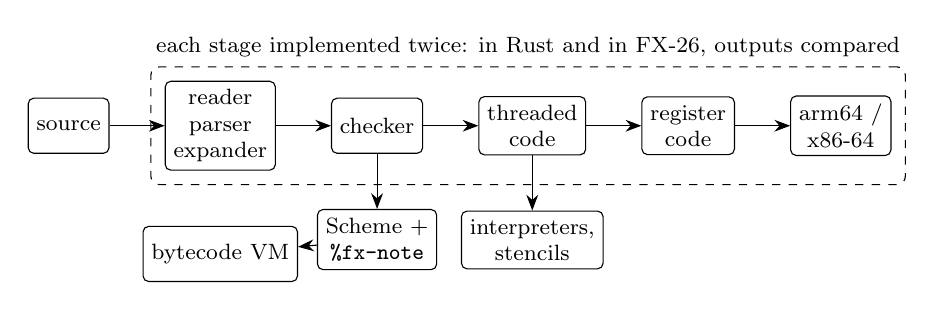
\begin{tikzpicture}[
  node distance=5mm and 7mm, font=\footnotesize,
  box/.style={draw, rounded corners=2pt, align=center, inner sep=3pt, minimum height=7mm},
  arr/.style={-{Stealth[length=2mm]}}]
\node[box] (src) {source};
\node[box, right=of src] (read) {reader\\parser\\expander};
\node[box, right=of read] (chk) {checker};
\node[box, right=of chk] (cw) {threaded\\code};
\node[box, right=of cw] (rc) {register\\code};
\node[box, right=of rc] (nat) {arm64 /\\x86-64};
\node[box, below=7mm of cw] (interp) {interpreters,\\stencils};
\node[box, below=7mm of chk] (scm) {Scheme +\\\texttt{\%fx-note}};
\node[box, below=7mm of read] (vm) {bytecode VM};
\draw[arr] (src) -- (read);
\draw[arr] (read) -- (chk);
\draw[arr] (chk) -- (cw);
\draw[arr] (cw) -- (rc);
\draw[arr] (rc) -- (nat);
\draw[arr] (cw) -- (interp);
\draw[arr] (chk) -- (scm);
\draw[arr] (scm) -- (vm);
\node[draw, dashed, rounded corners=3pt, inner sep=5pt,
      fit=(read)(chk)(cw)(rc)(nat),
      label={[font=\footnotesize]above:each stage implemented twice: in Rust and in \fx, outputs compared}] {};
\end{tikzpicture}
\Description{A pipeline from source through reader, checker, threaded code and register code to machine code.}
\caption{The Fixpt pipeline. Twelve named ``machines'' select a path
through it and which implementation performs each step.}
\label{fig:pipeline}
\end{figure}

\paragraph{Two front ends in lockstep.} Fixpt contains two complete
implementations of the pipeline in Figure~\ref{fig:pipeline}. One is
Rust (68,959 lines in the \fx{} crate's sources, plus 28,004 for native
code generation). The other is \fx{} (Table~\ref{tab:sizes}). Neither is
derived from the other. The command \cd{fixpt check} runs both checkers
and shows both results where they disagree; \cd{fixpt compile} compares
the two compilers' code; the test suite requires agreement of effect
summaries on every test program, of macro expansions, and---for the
code generator written in \fx{} against the Rust assembler---of machine
code word for word over the entire front end. The project rule is ``no
silent disagreements.'' Disagreements turned out to be a productive
source of bugs in both, and of specification: a feature is not done
until two programs written from one description agree about it.

\paragraph{Bootstrap.} The Rust compiler compiles the \fx{} front end
to register code and native code once and caches the result as a saved image of the heap (21~MB) keyed by a hash of the front end's source. Thereafter
programs are read, checked and compiled by the \fx{} front end; an
empty program runs in 50~ms. A fixed-point test checks that the
front end compiled by itself reproduces itself.

\paragraph{Code.} The checker's output is compiled to a \emph{threaded code} for a stack machine, and from there to \emph{register code}
with values in machine registers, and to native arm64 or x86-64 with
ordinary call frames. Twelve machines are kept runnable: the default
native one; interpreters of the threaded code in Rust and in
hand-assembled machine code; a copy-and-patch stencil
machine~\cite{copy-and-patch}; variants in which the \fx{} or the Rust
generator produces the code; a path that lowers to Scheme and runs on a
bytecode VM; and a metacircular evaluator. The simpler machines serve
as oracles: every benchmark is run on all of them with answers
cross-checked. Whatever the native compiler declines falls back to
threaded code through adapters.

\paragraph{Run time.} Values are 64-bit words with a three-bit tag.
The collector, in Rust, is a Cheney copying collector with a nursery
and a card-marking barrier; \cd{letrena} and \cd{letreap} regions are
arenas outside it. \cd{int} is arbitrary precision with a machine-word fast
path; fixed-width integers and floats are unboxed in registers. The
substrate is a Scheme engine that also hosts faithful
re-implementations of FX-87 and FX-91, which pass conformance corpora
recovered from the originals (161 of 161 programs parsing and 160 of
161 type-and-effect checking for FX-87; 182 of 182 for FX-91).

\begin{table}[t]
\caption{Sizes, in lines, measured at Fixpt commit \cd{0585488}
(2026-11-16), Kayak commit \cd{f59ac8cd} and Heist commit \cd{18efce5}.
Left: the \fx{} front end of Fixpt, written in \fx. Right: the other
bodies of \fx{} code.}
\label{tab:sizes}
\small
\begin{minipage}[t]{0.48\linewidth}
\begin{tabular}{@{}lrr@{}}
\toprule
Fixpt front end (in \fx) & files & lines\\
\midrule
checker & 104 & 32,529\\
native code generators & 38 & 18,263\\
macro expander & 27 & 13,288\\
compiler to threaded code & 17 & 5,603\\
register code & 14 & 5,203\\
parser, module loader & 7 & 4,036\\
evaluator & 5 & 2,744\\
reader & 6 & 1,025\\
linker, encoders, conventions & 7 & 2,511\\
other & 13 & 1,869\\
\midrule
total & 238 & 87,071\\
\bottomrule
\end{tabular}
\end{minipage}\hfill
\begin{minipage}[t]{0.48\linewidth}
\begin{tabular}{@{}lr@{}}
\toprule
Heist (applications) & lines\\
\midrule
ratfink, bounded model checker & 9,603\\
editor & 8,611\\
s7st, a Scheme implementation & 6,413\\
combo, SAT/SMT solver & 5,750\\
cfa, control-flow analysis & 3,423\\
casing, relational model finder & 2,725\\
kit, library & 701\\
\midrule
Kayak (in KFX) & \\
\midrule
KFX-to-Rust compiler & 24,755\\
\fx{} implementation & 16,133\\
threaded-code machine, tiers & 9,712\\
\bottomrule
\end{tabular}
\end{minipage}
\end{table}

%% ------------------------------------------------------------------
\section{Effects Choose the Rust: KFX}
\label{sec:kayak}

Kayak tests a claim implicit in \S\ref{sec:licences}: that \fx's types
and effects say enough about a program to compile it to a language
with a quite different discipline, without a run-time system that hides
the difference. KFX is a sublanguage of \fx{} under one invariant:
\emph{every KFX program is an \fx{} program with the same answer; KFX
may refuse \fx{} programs, never reinterpret them.} Its compiler,
written in KFX, emits safe Rust (the lint \cd{unsafe\_code = "deny"} is
the check).

\begin{table}[t]
\caption{How KFX reads Rust off \fx{} types and effects.}
\label{tab:kfx}
\small
\begin{tabular}{@{}ll@{}}
\toprule
\fx & Rust\\
\midrule
latent effect contains \cd{(goto $R$)} & \cd{fn} returns \cd{Result<T, Unwind>}; calls take \cd{?}\\
latent effect contains \cd{(comefrom $R$)} & \cd{async fn}; calls take \cd{.await}\\
effect-polymorphic procedure & \cd{async fn}, boxed per call\\
latent effect crosses processes (send, I/O, \ldots) & closure type gains \cd{Send + Sync}\\
\cd{letrena} region; region-polymorphic procedure & typed arena; lifetime parameter \cd{<'r>}\\
place parameter & \cd{<'p, P:\ Holds<T>>}\\
\cd{(ref $T$ $R$)} & \cd{\&Cell<T>} (never \cd{\&mut})\\
\cd{sumof}, \cd{productof}; \cd{define-generative} & generic enum, tuple struct; newtype\\
\cd{poly} over types & generics \cd{<A:\ Copy + 'static>}\\
\cd{moduleof} parameter & trait and type parameter\\
process, mailbox, I-cell; transmissible type & OS thread, \cd{Mutex}; \cd{Send + Sync}\\
self tail call & \cd{loop}\\
\bottomrule
\end{tabular}
\end{table}

\paragraph{Function colour is an effect.} Table~\ref{tab:kfx} gives the
mapping. The rows that matter are the first four. A language with
exceptions and coroutines compiled to Rust must ordinarily choose one
calling convention for every function, or compile each function
several ways. In KFX the choice is made per function by its latent
effect, which the checker already knows: only procedures that may abort
to a prompt return \cd{Result}; only procedures that may be suspended
are \cd{async}; ``nothing is compiled twice.'' A prompt whose body the
checker shows contains every abort gets an \cd{unreachable} arm. An
alternative design using unwinding panics was rejected on the stated
ground that then ``effects would decide nothing.'' Because a Rust
future resumes once, KFX exposes one-shot continuations only, and
multi-shot composable continuations are refused---one of three
permanent refusals, with untagged unions and pointer identity.

\paragraph{Where the two disciplines meet and part.} A \cd{letrena}
becomes a typed arena and its region variable a lifetime, after which
``Rust's borrow checker then refuses what \fx's refuses'': the two
systems agree on escape. They agree on transmissibility once the
closure rule above is added: Rust's \cd{Send} is about what a closure
\emph{holds}, \fx's rule about what it \emph{does}. They part on
aliasing. Effects do not become \cd{\&mut}: \fx{} dropped FX-87's
anti-aliasing rule, so a procedure may be instantiated with two region
parameters equal, and every KFX value is \cd{Copy}. The response on the
\fx{} side was an opt-in \cd{distinct} region binder; a mapping through
branded tokens~\cite{ghostcell} was studied and deferred.

\paragraph{The bootstrap.} There is no hand-written stage~0. Since a KFX
program is an \fx{} program, Fixpt runs the KFX compiler on its own
source; \cd{cargo} builds the Rust that results; and that binary, run on
the same source, must reproduce the Rust byte for byte. The loop closed
on the first day of the project with a 600-line compiler, and has been
required of every change since. The compiled compiler translates its
24,755 lines in well under a second; running the same compilation on
Fixpt as stage~0 was for some time 750 times slower (610~s), which
made Kayak Fixpt's most demanding performance client and drove that
figure to 9.5~s (\S\ref{sec:perf}).

Of 286 Fixpt test programs surveyed when KFX began, it accepted one;
the commonest first refusals were arbitrary-precision \cd{int} (48 programs),
\cd{define*} (43) and untyped definitions (36). It now accepts 194,
each agreeing with Fixpt's answer when run. K1 is tested, not proved,
and batches of adversarial probes (about 200 programs) repeatedly found
holes in it; the known remaining gaps are documented.

\paragraph{A second implementation.} Kayak also contains an
implementation of full \fx{} written in KFX: a checker, an interpreter
with a copying collector written in KFX, ports of Fixpt's compilers to
threaded code and register code, six execution tiers, and a REPL
written as \fx{} processes. Of 541 programs Fixpt's checkers accept,
Kayak's checker prints the same types for 423; of 386 Fixpt refuses,
Kayak accepts none; its register-code compiler emits words identical to
Fixpt's for 910 procedures of 917. \fx{} thus has three checkers
written by reading one description.

%% ------------------------------------------------------------------
\section{Experience}
\label{sec:eval}

This section reports what happened when \fx{} was used. It is an
experience report, and we state its limits before its contents.

\paragraph{What may be concluded.} That the discipline scales to
programs of tens of thousands of lines, including its own
implementation; how effect signatures are written when it does; what
the recorded costs to programmers were; and, for our own execution
strategies compared with one another, where the time goes.

\paragraph{What may not.}
\emph{Nothing here measures \fx{} against another language.} No
benchmark was timed on another implementation under controlled
conditions. The only external comparisons (\S\ref{sec:apps}) are two
applications against one Scheme system. Hardware is recorded only as
an Apple arm64 machine early on and a shared 128-core x86-64 Linux
machine later; runs are best-of-three or single, without variance;
optimisations were measured one at a time on eight small programs.
\emph{Nothing here measures programmer productivity or defects
prevented.} The applications were written by one author over three
weeks; the notes we draw on are qualitative; we have no measurement of
annotation overhead per line and no record of how often the checker
refused a program rightly or wrongly. The counts of
Table~\ref{tab:usage} describe one author's style.
\emph{The language is not finished.} Macros are a prototype (no local
macro bindings; soundness of signatures argued, not proved);
refinement of types by pattern matching on constructors, polymorphic
members of intersections, and static checking of one-shot
continuations are not built.

All figures are as recorded in the three repositories at the commits of
Table~\ref{tab:sizes}, with the date of each measurement.

\subsection{Programs and Their Signatures}
\label{sec:heist}

Table~\ref{tab:sizes} lists the code. Fixpt's own tests comprise 1,290
\fx{} programs and 1,160 Rust test functions; Heist's harness runs 211
trials, including 101 scripted terminal sessions of the editor; Kayak
keeps 865 \fx{} test programs and 3,442 recorded answers from Fixpt.

Heist is the cleanest evidence about use, because its author worked
\emph{with} the language rather than on it. Its six programs are
ports or reimplementations of existing systems: the editor descends
from a 13,000-line Scheme editor (119 of its 197 commands so far); the solver
of a Scheme CDCL/simplex/bit-blasting solver, to which it is
byte-identical on 800 fuzzed scripts; the model finder of Alloy~6's
semantics~\cite{alloy} (82 of 90 commands agree with Alloy 6.2.0, two
differ by design, six are inexpressible there); the Scheme passes
thirteen library test suites for the Scheme standard, the \cd{base}
library's 1,078 tests among them.

\begin{table}[t]
\caption{How effects are written in Heist's 37,226 lines of
application source (tests excluded; comments and strings stripped).}
\label{tab:usage}
\small
\begin{minipage}[t]{0.50\linewidth}
\begin{tabular}{@{}lr@{}}
\toprule
\cd{subr} signatures & 3,893\\
\midrule
\quad effect is a named effect or variable & 2,564 (66\%)\\
\quad effect is explicit and contains \cd{spin} & 615 (16\%)\\
\quad effect is \cd{pure} & 497 (13\%)\\
\quad effect is explicit, without \cd{spin} & 217 (6\%)\\
\midrule
\cd{define*} / \cd{define} & 1,756 / 1,728\\
\cd{define-type} & 456\\
\cd{(the $T$ $e$)} ascriptions & 663\\
\cd{acyclic} & 1,346\\
\bottomrule
\end{tabular}
\end{minipage}\hfill
\begin{minipage}[t]{0.46\linewidth}
\begin{tabular}{@{}lr@{}}
\toprule
form & uses\\
\midrule
\cd{tagcase} (match on a sum) & 1,301\\
\cd{load-module}, \cd{load-moduleof} & 464\\
\cd{define-syntax} & 70\\
\cd{poly} / \cd{plambda} & 53 / 52\\
\cd{module-parameters} & 53\\
\cd{oneof} & 34\\
prompts, composable continuations & 6\\
\cd{pselect}, \cd{attempt}, \cd{stage} & 2, 1, 1\\
\cd{mu}, \cd{allof}, \cd{spawn}, \cd{par}, \cd{letregion} & 0\\
\bottomrule
\end{tabular}
\end{minipage}
\end{table}

Table~\ref{tab:usage} counts forms in Heist's sources. Three
observations follow.

\emph{Effects are named, not written.} Two thirds of all procedure
types carry an effect \emph{abbreviation}; each program defines one
region for its state and one effect for ``what this program does''
(\cd{cb-eff} appears 687 times in the solver). Explicit \cd{maxeff}
occurs only 300 times in 37,000 lines. Signatures did not grow the long
effect rows that are the usual objection to declared effects, but the
price is precision: every named effect of the five programs includes
\cd{spin}, so most application procedures do not claim termination. The exception is
instructive---the shared library is polymorphic and precise,
\begin{lstlisting}
(define map
  (poly ((p place) (a type) (b type) (e effect) (r region))
    (subr (maxeff e (read (acyclic p)) (alloc r))
          ((subr e (a) b) (listof a (acyclic p))) (listof b r)))
  ...)
\end{lstlisting}
and no procedure in it says \cd{spin}. Precision pays where code is
reused and is abandoned where it is not.

\emph{Inferring the globals is essential.} Half of all definitions use
\cd{define*}. Without it, calling a library procedure from a \cd{pure}
definition is refused, since the callee is a global.

\emph{The advanced type features are used by the language's
implementers, not its clients.} Heist uses no \cd{mu}, no intersection,
no \cd{letregion}, and none of the process forms (the editor implements
its own actors over \cd{pselect}); recursive types arrive through named
\cd{define-type}s. Module parameters, tagged sums and delimited control
(the Scheme's \cd{call/cc}, \cd{dynamic-wind} and time slices; the
model checker's backtracking) carry the weight.

\subsection{What the Discipline Enabled, Cost and Caught}

\paragraph{Enabled.} Besides rollback by \cd{attempt}
(\S\ref{sec:conc}), the control-flow analysis benefits directly from
the types: nearly every standard procedure is first-order, and on the
editor's twenty files only 83 of 8,800 flow notes hold an unknown
value, with a deeper context changing none. The analysis reports
regions and effects (``\cd{calls make-box; effect (alloc @ed)}''), not
only values. The model checker turns a procedure with \cd{requires}
and \cd{ensures} into a modular proof obligation over symbolic values.

\paragraph{Cost.} The recorded friction is specific. \emph{Region
annotations}: after adopting the shared list library, the model checker
needed 101 ascriptions \cd{(the (listof $T$ acyclic) \ldots)} at 366
call sites, until the default of \S\ref{sec:core} removed all of them.
\emph{Termination}: loops the checker cannot see end (\cd{gcd},
sorting, exponentiation) were given a fuel parameter to remain
\cd{pure}. \emph{Cancellability}: because \cd{attempt} forbids writes,
the solver makes errors values, and the editor returns actions as data.
\emph{Messages}: types of parameterised modules print fully expanded
and run to pages. And 663 ascriptions remain, ``more often than one
would like.''

\paragraph{Caught.} We cannot report a count of defects the checker
found in application code: none was recorded as such. What is recorded
runs the other way: tightening the checker (requiring \cd{spin} where
an effect reads all globals) exposed eight wrongly declared effects in
the editor, one of them a \cd{pure} that was not; and the application
effort found a soundness hole in the language (\S\ref{sec:core}).

\paragraph{Clients shaped the language.} Dated entries in the language
document attribute features to the client that asked. From Heist:
\cd{attempt} and \cd{attempt-within}, child processes and the
\cd{(io process)} effect, \cd{pselect} arms for process events, staged
code compiled natively and staged against a sealed module, module
parameters of every kind, the acyclic region default, and inline
region allocation. From Kayak: processes, \cd{par}, \cd{pselect} and
monitors; the \cd{io} effect family with errors as values (so that
KFX's invariant stays checkable for programs that perform I/O); a
syscall interface; code a program makes; and \cd{distinct} regions.

\subsection{Execution Strategies Compared with One Another}
\label{sec:perf}

\begin{table}[t]
\caption{Run time in milliseconds (best of three) of the eight
per-commit benchmarks on seven of the machines; arm64, 2026-09-28.
``Lowered'' is Scheme on the bytecode VM; ``rust'' and ``hand'' are
interpreters of threaded code; ``compiled'' is threaded code compiled
to machine code; ``registers'' is register code in the threaded machine's calling convention; ``native'' uses machine call frames.}
\label{tab:machines}
\small
\begin{tabular}{@{}lrrrrrrr@{}}
\toprule
 & lowered & rust & hand & stencils & compiled & registers & native\\
\midrule
captures & 111.8 & 49.1 & 14.6 & 14.5 & 12.4 & 9.2 & 21.9\\
closures & 343.2 & 699.4 & 75.7 & 85.0 & 60.3 & 17.6 & 24.0\\
fib (30) & 180.5 & 213.7 & 16.1 & 22.0 & 13.5 & 4.9 & 2.4\\
helpers & 865.5 & 1274.3 & 89.3 & 110.0 & 55.2 & 2.8 & 2.3\\
lists-region & 332.8 & 314.4 & 96.9 & 111.8 & 82.8 & 7.2 & 156.5\\
lists & 297.8 & 470.1 & 54.7 & 65.9 & 47.4 & 8.5 & 10.5\\
loop & 736.0 & 452.2 & 64.5 & 89.7 & 41.2 & 4.7 & 4.3\\
tak & 51.6 & 78.0 & 6.6 & 8.7 & 4.5 & 1.7 & 1.2\\
\bottomrule
\end{tabular}
\end{table}

Fixpt can run a program twelve ways, from a bytecode interpreter to
native code. Table~\ref{tab:machines} compares seven of them on eight
small programs; it is the most recent complete such table, and it says
how much each stage of compilation contributes, not how \fx{} compares
with anything else. The spread from a bytecode VM to native code is 5--380
times on these programs; the stencil machine does not improve on the
hand-written threaded interpreter; register code is where most of the
gain arrives. (Two outliers in the ``native'' column, \cd{captures}
and \cd{lists-region}, predate later work: \cd{lists-region} was
subsequently measured at 7.0~ms once region allocation was inlined in
that convention.)

\paragraph{What types, effects and regions contribute.} The recorded
before-and-after measurements are per optimisation:
\begin{itemize}
\item \emph{Typed calls} (no closure test): 2--12\%.
  \emph{Typed primitives} (no tag tests): 6--20\% on \cd{loop},
  within noise elsewhere.
\item \emph{Effect summaries} (one guarded version per body where the
  procedure cannot redefine globals): \cd{helpers} from 9.0 to 2.8~ms
  as register code and from 6.1 to 2.0~ms native.
\item \emph{Regions}: allocating list cells inline in a \cd{letrena}
  arena took \cd{lists-region} to 8.1~ms against 12.4~ms for the same
  program on the collected heap as register code; inline region
  allocation of references and arrays, requested for the Scheme's
  environment frames, was about eight-fold (487 to 58~ms per $10^7$
  allocations).
\item \emph{Checked notes} on the lowering path: 1.21 times over the
  compiled engine without them, best of five.
\end{itemize}
Two candidate optimisations that effects would license were measured
and \emph{not} built: common-subexpression elimination of pure calls
(109 opportunities in the front end, none in the benchmarks) and
loop-invariant lifting (3). We report these because the rule of
\S\ref{sec:intro} applies to optimisations too.

\paragraph{Suites.} We ported 53 of the 75 programs of a standard Scheme benchmark suite (the rest need floating point or file I/O not then
available) and 46 programs from MLton's benchmarks, OCaml's test-suite
classics and Sandmark's Benchmarks Game. The ports were used to
find performance cliffs---arbitrary-precision \cd{int} without a machine-word fast path;
sums and products built out of line (\cd{mlton/peek} improved 4.8
times)---rather than timed under controlled conditions; the recorded
single-run times include one to three seconds of start-up that has
since been removed, and we do not tabulate them.

\paragraph{Compile time.} Compiling itself (2026-10-02, then-current
sizes), the \fx{} checker took 1,385~ms against 394~ms for the Rust
checker on the same input (3.5 times), the \fx{} compiler to threaded code 757~ms against 70~ms (11 times), and the \fx{} code generator
979~ms against 7~ms. Self-hosting is paid for; the price is in the
open. Kayak's 30,000-line compiler is the standing workload: checking,
compiling and running it as stage~0 went from 610~s to 9.5~s in three
weeks; in an earlier measurement it loaded from its compiled form in
1.15~s against 3.30~s from source.

\paragraph{KFX as Rust.} On the day KFX first ran the per-commit
programs, its Rust ran \cd{fib} in 1.2~ms against 2.6~ms for Fixpt's
fastest machine of the time, \cd{tak} in 0.5 against 1.0, \cd{lists}
in 5.4 against 6.0, and \cd{closures} in 21 against 14 (closures are
leaked \cd{dyn Fn}). Records with declared layout matched hand-written
\cd{\#[repr(C)]} Rust (10.5 and 5.0~ms against 10.4 and 4.9).

\subsection{Two Applications against a Scheme System}
\label{sec:apps}

\begin{table}[t]
\caption{Heist applications against the Scheme systems they were
ported from or compete with. Left: the SAT/SMT solver against its
original running on Larceny, a native-code Scheme compiler (2026-10-28,
x86-64 Linux). Right: Heist's Scheme, as an interpreter and compiling
to \fx{} at run time by \cd{stage},
against Larceny's interpreter and compiler (2026-10-31; ms).}
\label{tab:apps}
\small
\begin{minipage}[t]{0.40\linewidth}
\begin{tabular}{@{}lrr@{}}
\toprule
 & original & \fx\\
\midrule
par16-2 & 0.23 s & 0.71 s\\
bmc-ibm-12 & 3.1 s & 4.6 s\\
bmc-galileo-8 & 1.3 s & 1.8 s\\
QF\_LRA solved & 56/56 & 56/56\\
QF\_LIA solved & 96/106 & 94/106\\
QF\_BV solved & 109/125 & 109/125\\
start-up & 0.05 s & 0.29 s\\
\bottomrule
\end{tabular}
\end{minipage}\hfill
\begin{minipage}[t]{0.58\linewidth}
\begin{tabular}{@{}lrrrr@{}}
\toprule
 & \multicolumn{2}{c}{s7st on \fx} & \multicolumn{2}{c}{Larceny}\\
  & interp. & staged & interp. & compiled\\
\midrule
\cd{(fib 25)} & 49.5 & 7.1 & 11.3 & 0.5\\
\cd{(tak 18 12 6)} & 12.0 & 1.7 & 4.0 & 0.1\\
named-let loop, $10^6$ & 108.8 & 25.0 & 52.9 & 1.1\\
\cd{map} over 200k & 250.1 & 93.7 & 34.7 & 12.6\\
\cd{do} over vector, 500k & 68.0 & 20.4 & 31.1 & 1.4\\
countdown, $10^7$ & 661.9 & 243.8 & 244.1 & 6.6\\
\bottomrule
\end{tabular}
\end{minipage}
\end{table}

Table~\ref{tab:apps} gives the only two comparisons with another system that exist. The solver,
a statically typed port performing the same search, is 1.4 to 3 times
slower than its dynamically typed original on a mature native-code
Scheme. The Scheme implemented \emph{in} \fx{} is, once it compiles to
\fx{} through \cd{stage}, between Larceny's interpreter and its
compiler: a dynamically typed language hosted on a typed one pays for
its uniform representation in the host's sums. The editor is the
favourable case: 8~$\mu$s per key in a burst and 0.4~ms for an
isolated key, against 1.5~ms recorded for its predecessor on Larceny,
with \cd{attempt} around each command costing 1.7~$\mu$s. The model
finder runs its 90 cross-check commands in 17~s; the control-flow
analysis covers the editor's 9,855 notes in 1.8~s including start-up.
Start-up from separately compiled files is 0.1--1.2~s per program (median of 20), or 30~ms from a saved image of the heap.

%% ------------------------------------------------------------------
\section{Soundness, as Practised}
\label{sec:soundness}

\paragraph{What is on paper.} K26 is a declarative calculus for the
memory and control fragment with a small-step semantics over a store,
a stack of places with tombstones for freed arenas, and evaluation
contexts with region, place, freeze and prompt frames. Implicit
masking is not preserved by reduction, so the calculus elaborates it
into two explicit binders, one for each way a region can be private.
For this calculus, progress and preservation are proved in the
syntactic style~\cite{wright-felleisen}, with corollaries that no freed
place is accessed, that frozen regions are never written and data at
them is acyclic, and that sizes are respected. Effect soundness and
erasure of specifications are sketched. \emph{Termination of
\cd{spin}-free programs is conjectured}; it needs a step-indexed Kripke
logical relation that has not been written. Nothing is mechanised, and
the calculus has not been extended to unions, intersections, I/O or
processes; the subtyping lemma must be redone for unions and
intersections~\cite{muehlboeck-tate}.

\paragraph{What was found.} Alongside the proof effort, hand-written
probe programs were run against both checkers under a step limit.
Eighteen findings were recorded (Table~\ref{tab:findings}); all are
fixed. Eight concern \cd{spin}. The pattern is that \emph{every way of
tying a knot is a way to loop}, and a termination effect must find
them all: self-application through a recursive type (\cd{(w w)} was
accepted as \cd{pure} when the parameter shadowed a known name);
through a type binder; through the store; through a continuation saved
in a private I-cell and re-entered, whose effects masking had
correctly removed---but whose divergence it must not. Two findings
were memory-unsafe, one demonstrated: a closure whose type no longer
mentioned an arena escaped it and later read reused memory. One was a
type unsoundness from intersections and allocation (one cell at two
types).

\begin{table}[t]
\caption{Soundness findings, by what was violated.}
\label{tab:findings}
\small
\begin{tabular}{@{}llr@{}}
\toprule
violated & findings & count\\
\midrule
\cd{spin}: a program typed as terminating diverges & F1, F3, F5, F8, F9, F11, F15, F17 & 8\\
sizes and naturals & F4, F10, F16 & 3\\
memory safety (regions, arenas) & F2, F13 & 2\\
type safety (intersection with effects) & F18 & 1\\
compiler or run time disagrees with checker & F6, F7, F12, F14 & 4\\
\bottomrule
\end{tabular}
\end{table}

One statement in the development is known to be false as written:
effect soundness for composable continuations, since a continuation's
frames can touch a region that was private to the context that
captured it. We judge it harmless because every call of a composable
continuation carries control effects, but the theorem needs restating.

\paragraph{What we take from it.} Two independent checkers agreeing is
strong evidence about the \emph{specification's clarity} and no
evidence about its \emph{soundness}: the masking hole of
\S\ref{sec:core} was faithfully implemented twice. The fixes for the two most recent findings are ``argued, not
proved.'' An application author has proposed a sanitising machine,
systematic enumeration of small programs, and a mechanised model in
Rocq with Iris; we regard a mechanised proof of the masking rule with
\cd{spin} and control as the most valuable piece of future work on the
language.

%% ------------------------------------------------------------------
\section{Related Work}
\label{sec:related}

\paragraph{The FX line.} \fx{} takes FX-87's region-indexed types,
explicit signatures and masking~\cite{fx87,lucassen-gifford,lucassen-thesis};
the control effects of Jouvelot and Gifford~\cite{jouvelot-gifford};
and FX-91's first-class modules and local inference
machinery~\cite{fx91,sheldon-gifford}. It does not take effect
reconstruction~\cite{jouvelot-gifford-reconstruction,talpin-jouvelot}:
inference is local, and whole effects are inferred only on request.
Reistad and Gifford's cost effects~\cite{reistad-gifford} are a
direction we have not followed. Its departures from the line are
immutable sums, equi-recursive types, generativity separated from
modules, and everything in \S\ref{sec:licences}.

\paragraph{Regions.} Tofte and Talpin~\cite{tofte-talpin} infer
regions for memory management; Cyclone~\cite{cyclone} declares them.
\fx's regions are primarily units of \emph{effect}: most data lives on
a collected heap, a region need not have a lifetime, and arenas are an
opt-in. Freezing a region to obtain acyclicity and covariance relates
to reference immutability~\cite{gordon-uniqueness}.

\paragraph{Effect handlers and capabilities.} Koka~\cite{koka},
Frank~\cite{frank}, Effekt~\cite{effekt} and OCaml~5~\cite{ocaml5}
centre on user-defined effects with handlers; Koka also tracks
divergence, without attempting to prove termination by size change.
Flix~\cite{flix} uses Boolean unification for effect polymorphism and
region-scoped mutation. Capture checking~\cite{capturing-types} and
reachability types~\cite{reachability} track what closures hold. \fx{}
has no user-defined effects: its atoms are fixed because each has a
consumer built for it. Delimited control with typed prompt tags plays
the role handlers play elsewhere. Whether licences can be given for
user-defined effects is open.

\paragraph{Effects for optimisation and parallelism.} That effect
information licenses optimisation and parallel evaluation was FX's
original motivation; non-interference follows
Reynolds~\cite{reynolds-interference}. Our contribution is breadth of
consumers in one system, and speculative evaluation in an interactive
front end, of which we know no precedent.

\paragraph{Structural types.} Recursive subtyping follows
\cite{amadio-cardelli,brandt-henglein}; narrowing follows Typed
Racket~\cite{typed-scheme,logical-types}; intersections with effects
follow the restriction of Davies and Pfenning~\cite{davies-pfenning};
bidirectional checking~\cite{local-type-inference,bidir-survey}.

\paragraph{Macros and modules.} Typed macros follow
Herman~\cite{herman-wand,herman-thesis}; inference follows
\cite{inferring-scope}; hygiene by renaming follows
\cite{clinger-rees,hanson,clinger-er}. Scope-set expansion~\cite{sets-of-scopes}
and syntax-parse~\cite{fortifying-macros} offer error reporting in the
user's terms by other means, without static binding signatures.
Dependent procedure types over modules predate, and are generalised
by, the ML line through F-ing modules and 1ML~\cite{leroy-applicative,f-ing,oneml}.

\paragraph{Compiling to Rust, and self-hosting.} We know of no prior
translation that selects among Rust's function colours by a source
effect system. Maintaining two implementations of a language so that
each checks the other is old practice in compiler bootstrapping; doing
so for the type checker, per program and in the user's tools, is the
part we found most valuable.

%% ------------------------------------------------------------------
\section{Conclusion}

Effects on regions, declared in signatures and masked where
unobservable, scale to a language that implements itself and to
applications written by people who did not design it---provided that
effects can be named, that the globals a body reads are computed, and
that regions default sensibly. The discipline pays when effect
information is consumed: every consumer in \S\ref{sec:licences} is a
few lines stating a condition on effects, and each replaces a
mechanism (a trusted purity annotation, a sandbox for speculative
evaluation, a transactional log for rollback, a uniform calling
convention for unwinding) that systems without effects must build or
do without. The hard part is the termination effect, which is the
most useful to consumers and the easiest to get wrong; it accounts for
almost half of what we got wrong.

\fx, Fixpt, Heist and Kayak are open source.

\bibliographystyle{ACM-Reference-Format}
\bibliography{fx26}

\end{document}
